\documentclass[aspectratio=169]{beamer}
\usetheme{TUDelft}

% ====================================================================
% ANIMATION TOGGLE
% ====================================================================
\newif\ifanimated
\animatedtrue
\ifdefined\staticmode
  \animatedfalse
\fi
\newcommand{\cpause}{\ifanimated\pause\fi}

% Packages
\usepackage{amsmath}
\usepackage{amssymb}
\usepackage{pifont}
\usepackage{graphicx}
\usepackage{tikz}
\usepackage{booktabs}
\usepackage{listings}
\usepackage{xcolor}
\usepackage{tcolorbox}
\usepackage{bm}

% Python code styling
\lstset{
    language=Python,
    basicstyle=\ttfamily\footnotesize,
    keywordstyle=\color{blue},
    commentstyle=\color{gray},
    stringstyle=\color{red},
    showstringspaces=false,
    breaklines=true,
    frame=single,
    numbers=left,
    numberstyle=\tiny\color{gray}
}

% TikZ libraries
\usetikzlibrary{shapes,arrows,arrows.meta,positioning,calc,decorations.pathreplacing,fit,backgrounds,matrix}

% Custom colors
\definecolor{sparse}{RGB}{52,152,219}    % Blue
\definecolor{dense}{RGB}{231,76,60}      % Red
\definecolor{hybrid}{RGB}{46,204,113}    % Green

% Math shortcuts
\newcommand{\vq}{\mathbf{q}}
\newcommand{\vp}{\mathbf{p}}
\newcommand{\vd}{\mathbf{d}}
\newcommand{\vk}{\mathbf{k}}
\newcommand{\vv}{\mathbf{v}}
\DeclareMathOperator*{\argmax}{arg\,max}

% Import theme macros
\usepackage{tikz}
\usetikzlibrary{positioning, shapes, arrows, shadows, fit, calc, decorations.pathreplacing}

% Semantic Colors - One meaning per color
\definecolor{irSparse}{HTML}{3498DB}   % Sparse/BM25: Blue
\definecolor{irDense}{HTML}{E67E22}    % Dense/Embeddings: Orange
\definecolor{irRerank}{HTML}{C0392B}   % Rerank/Cross-encoder: Red
\definecolor{irHybrid}{HTML}{2ECC71}   % Hybrid/Fusion: Green
\definecolor{irANN}{HTML}{9B59B6}      % ANN/Infra: Purple
\definecolor{irInfra}{HTML}{58595B}    % General Infra: Dark Gray
\definecolor{irMuted}{HTML}{D9D9D9}    % Faint Gray

% Base Styles - Consistent Diagram Grammar
\tikzset{
    irBoxBase/.style={
        rectangle, 
        draw, 
        rounded corners=2pt, 
        minimum height=0.8cm, 
        minimum width=2cm,
        font=\small\sffamily,
        align=center,
        drop shadow={opacity=0.15},
        inner sep=5pt
    },
    irDatabase/.style={
        cylinder, 
        draw, 
        shape border rotate=90, 
        aspect=0.25, 
        minimum height=1.2cm, 
        minimum width=1cm,
        fill=irMuted!20,
        draw=irInfra,
        font=\tiny\sffamily,
        align=center
    },
    % Semantic Variants
    sparse/.style={irBoxBase, fill=irSparse!10, draw=irSparse},
    dense/.style={irBoxBase, fill=irDense!10, draw=irDense},
    rerank/.style={irBoxBase, fill=irRerank!10, draw=irRerank},
    hybrid/.style={irBoxBase, fill=irHybrid!10, draw=irHybrid},
    ann/.style={irBoxBase, fill=irANN!10, draw=irANN},
    infra/.style={irBoxBase, fill=irInfra!10, draw=irInfra},
    % Legacy support / Utility
    muted/.style={irBoxBase, fill=irMuted!20, draw=irMuted!80!black, text=irMuted!50!black},
    ghost/.style={irBoxBase, fill=white, draw=irMuted!50, text=irMuted, dashed, drop shadow={opacity=0}},
    emph/.style={draw=irRerank, thick, drop shadow={shadow xshift=0mm, shadow yshift=0mm, fill=irRerank, opacity=0.3}},
    % Arrows
    irArrowBase/.style={->, thick, >=latex, draw=irInfra},
    irLabel/.style={
        font=\tiny\itshape, 
        text=irInfra, 
        align=center, 
        text width=2.5cm, 
        inner sep=3pt
    }
}


% =========================================================
% Stage Badge System
% =========================================================
% \irStage{StageName}
\newcommand{\irStage}[1]{%
    \begin{tikzpicture}[remember picture, overlay]
        \node[
            anchor=north east,
            fill=irInfra!10,
            text=irInfra,
            font=\tiny\bfseries,
            inner sep=3pt,
            rounded corners=1pt,
            yshift=-0.5cm,
            xshift=-0.5cm
        ] at (current page.north east) {#1};
    \end{tikzpicture}%
}

% =========================================================
% Math Highlighting
% =========================================================
% \mathhl[color]{content}
\newcommand{\mathhl}[2][irDense!30]{%
    \colorbox{#1}{$\displaystyle #2$}%
}

% =========================================================
% Math Vectors
% =========================================================
\newcommand{\vs}{\mathbf{s}}

% =========================================================
% Core Box Primitives
% =========================================================
% \IRBox[width]{id}{at}{title}{subtitle}{variant}
% Default width chosen for lecture slides; override when needed.
% \IRBox[width]{id}{at}{title}{subtitle}{variant}[extra options]
\DeclareDocumentCommand{\IRBox}{O{3.5cm} m m m m m O{}}{%
    \node[#6, text width=#1, #7] (#2) at #3 {%
        \textbf{#4}%
        \if\relax\detokenize{#5}\relax
        \else\\[-1mm]\scriptsize #5%
        \fi
    };%
}

% \IRWideBox{id}{at}{width}{title}{subtitle}{variant}
\newcommand{\IRWideBox}[6]{%
    \node[#6, text width=#3] (#1) at #2 {%
        \textbf{#4}%
        \if\relax\detokenize{#5}\relax
        \else\\[-1mm]\scriptsize #5%
        \fi
    };%
}

% =========================================================
% Arrow Primitives
% =========================================================
% Safe default: left-to-right flow
% \IRArrow{from}{to}{label}
\newcommand{\IRArrow}[3]{%
    \draw[irArrowBase] (#1.east) -- node[irArrowLabelAbove] {#3} (#2.west);%
}

% Explicit left-to-right
% \IRArrowLR{from}{to}{label}
\newcommand{\IRArrowLR}[3]{%
    \draw[irArrowBase] (#1.east) -- node[irArrowLabelAbove] {#3} (#2.west);%
}

% Explicit top-to-bottom
% \IRArrowTB{from}{to}{label}
\newcommand{\IRArrowTB}[3]{%
    \draw[irArrowBase] (#1.south) -- node[irArrowLabelRight] {#3} (#2.north);%
}

% Fully explicit anchor-to-anchor path
% \IRArrowPath{from anchor}{to anchor}{label}
% Example: \IRArrowPath{a.east}{b.north}{score}
\newcommand{\IRArrowPath}[3]{%
    \draw[irArrowBase] (#1) -- node[irArrowLabelAbove] {#3} (#2);%
}

% Orthogonal elbow path
% \IRArrowElbow{from anchor}{to anchor}{label}
% Example: \IRArrowElbow{a.east}{b.north}{feedback}
\newcommand{\IRArrowElbow}[3]{%
    \draw[irArrowBase] (#1) -| node[irArrowLabelBox] {#3} (#2);%
}

% Slanted arrow for special cases only
% \IRArrowSlanted{from anchor}{to anchor}{label}{pos}{width}
\newcommand{\IRArrowSlanted}[5]{%
    \draw[irArrowBase] (#1) -- node[above, sloped, irLabel, pos=#4, text width=#5, fill=white, inner sep=1pt] {#3} (#2);%
}

% =========================================================
% Accent Elements
% =========================================================
% \IRBadge{at}{text}
\newcommand{\IRBadge}[2]{%
    \node[
        draw=irAccent,
        fill=irAccent!20,
        rounded corners=1pt,
        font=\tiny\bfseries,
        inner sep=2pt
    ] at #1 {#2};%
}

% =========================================================
% Grouping
% =========================================================
% \IRGroup{fit nodes}{label}{variant}
% Example: \IRGroup{(a)(b)(c)}{First-stage retrieval}{muted}
\newcommand{\IRGroup}[3]{%
    \node[
        irGroupBase,
        #3,
        fit=#1
    ] (group) {};
    \node[
        anchor=north west,
        font=\tiny\bfseries,
        #3
    ] at ([xshift=2pt,yshift=-2pt] group.north west) {#2};%
}

% =========================================================
% Domain-Specific Shapes
% =========================================================
% \IRDocStack{id}{at}{label}
\newcommand{\IRDocStack}[3]{%
    \node[irDocStack] (#1) at #2 {#3};%
}

% \IRDatabase{id}{at}{label}
\newcommand{\IRDatabase}[3]{%
    \node[irDatabase] (#1) at #2 {#3};%
}

% =========================================================
% Layout Helpers
% =========================================================
% \IRPipelineTier{id}{at}{text}{label}{variant}
\newcommand{\IRPipelineTier}[5]{%
    \IRBox{#1}{#2}{#3}{}{#5}[]
    \node[anchor=west, irLabel, xshift=0.5cm] at (#1.east) {#4};%
}

% \IRTelescopeTier{id}{at}{width}{text}{variant}
\newcommand{\IRTelescopeTier}[5]{%
    \node[
        irTelescopeBase,
        #5,
        minimum width=#3
    ] (#1) at #2 {#4};%
}

% \IRStep{id}{at}{title}{subtitle}{variant}
% Creates a numbered step badge left of a box.
\newcommand{\IRStep}[5]{%
    \node[
        circle,
        draw=irAccent,
        fill=irAccent!20,
        font=\tiny\bfseries,
        inner sep=2pt
    ] (#1_num) at #2 {#1};
    \node[
        #5,
        text width=3.5cm,
        right=1.5cm of #1_num
    ] (#1) {%
        \textbf{#3}%
        \if\relax\detokenize{#4}\relax
        \else\\[-1mm]\scriptsize #4%
        \fi
    };
    \draw[irArrowBase, thin] (#1_num.east) -- (#1.west);%
}


% Title information
\title[Dense Retrieval]{Representation Learning for Rankings}
\subtitle{Lecture 5: Dense Retrieval --- From Bi-Encoders to Late Interaction}
\author{Avishek Anand}
\institute{Information Retrieval}
\date{\today}

% Automatic Roadmap/Outline slide at the start of each section
\AtBeginSection[]
{
  \begin{frame}{Roadmap}
    \tableofcontents[currentsection]
  \end{frame}
}

\begin{document}

% Title slide
\begin{frame}
\titlepage
\end{frame}

\begin{frame}{Outline}
\tableofcontents
\end{frame}

% ====================================================================
\section{Recap \& Motivation --- From Re-ranking to Retrieval}
% ====================================================================

\begin{frame}[plain]
\sectionpage
\end{frame}

\begin{frame}{Recap: Where We Are}
\begin{block}{What We've Built So Far}
\begin{itemize}
    \item \textbf{Lecture 2:} Inverted indexes and ANN indexes (IVF+PQ, HNSW)
    \item \textbf{Lecture 5:} BM25, Language Models, RM3 for scoring and expansion
    \item \textbf{Lecture 6:} BERT cross-encoders for re-ranking (monoBERT, monoT5)
\end{itemize}\cpause
\end{block}

\vspace{1em}

\begin{alertblock}{The Remaining Problem}
Cross-encoders are \textbf{too slow for retrieval}:
\begin{itemize}
    \item Re-ranking 100 docs: 0.5s \textcolor{green}{\checkmark} \quad Full corpus (8.8M): 12+ hours \textcolor{red}{\ding{55}}
    \item BM25 misses semantic matches: ``automobile issues'' vs.\ ``car problems''
    \item Bounded Recall: if retriever misses a relevant doc, the cross-encoder can \textbf{never} recover it
\end{itemize}
\end{alertblock}
\end{frame}

\begin{frame}{Today's Goal}
\begin{exampleblock}{The Missing Piece}
Combine the \textbf{semantic understanding} of BERT with the \textbf{retrieval speed} of ANN indexes from Lecture 2.
\end{exampleblock}

\vspace{1em}

\begin{block}{Key Idea: The Bi-Encoder}
\begin{enumerate}
    \item Encode all documents \textbf{offline} with BERT $\to$ dense vectors
    \item Store in ANN index (IVF+PQ from Lecture 2!)
    \item At query time: encode query with BERT $\to$ ANN search $\to$ top-$k$
\end{enumerate}
\end{block}

\cpause
\vspace{0.5em}

\begin{alertblock}{The Trade-off}
Bi-encoders are \textbf{less accurate} than cross-encoders (no query-document interaction) but \textbf{fast enough for full-corpus retrieval}.
\end{alertblock}
\end{frame}

\begin{frame}{The Dense Retrieval Pipeline}
\begin{center}
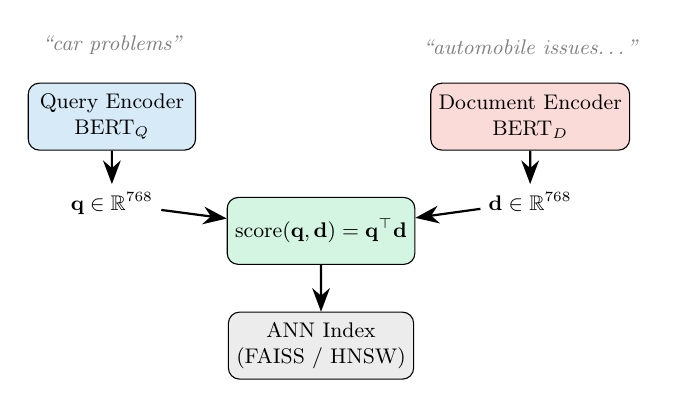
\begin{tikzpicture}[
    scale=0.85, transform shape,
    box/.style={draw, rounded corners, minimum height=1cm, minimum width=2.5cm, align=center, font=\small},
    arr/.style={-{Stealth[length=3mm]}, thick}
]
\node[box, fill=sparse!20] (qenc) {Query Encoder\\$\text{BERT}_Q$};
\node[box, fill=dense!20, right=3.5cm of qenc] (denc) {Document Encoder\\$\text{BERT}_D$};
\node[below=0.5cm of qenc, font=\small] (q) {$\vq \in \mathbb{R}^{768}$};
\node[below=0.5cm of denc, font=\small] (d) {$\vd \in \mathbb{R}^{768}$};
\node[box, fill=hybrid!20, below=1.2cm of $(qenc)!0.5!(denc)$] (sim) {$\text{score}(\vq,\vd) = \vq^\top \vd$};
\node[box, fill=gray!15, below=0.7cm of sim] (ann) {ANN Index\\(FAISS / HNSW)};

\draw[arr] (qenc) -- (q);
\draw[arr] (denc) -- (d);
\draw[arr] (q) -- (sim);
\draw[arr] (d) -- (sim);
\draw[arr] (sim) -- (ann);

\node[above=0.3cm of qenc, font=\small\itshape, text=gray] {``car problems''};
\node[above=0.3cm of denc, font=\small\itshape, text=gray] {``automobile issues\ldots''};
\end{tikzpicture}
\end{center}

\vspace{0.2em}

\begin{columns}
\begin{column}{0.48\textwidth}
\textbf{Offline (once):}
\begin{itemize}
    \item Encode all 8.8M passages
    \item Build ANN index
    \item $\sim$hours on GPU
\end{itemize}\cpause
\end{column}
\begin{column}{0.48\textwidth}
\textbf{Online (per query):}
\begin{itemize}
    \item Encode query: $\sim$5 ms
    \item ANN search: $\sim$10 ms
    \item Total: $\sim$15 ms \textcolor{green}{\checkmark}
\end{itemize}
\end{column}
\end{columns}
\end{frame}

\begin{frame}{Cross-Encoder vs.\ Bi-Encoder: Architecture}
\begin{center}
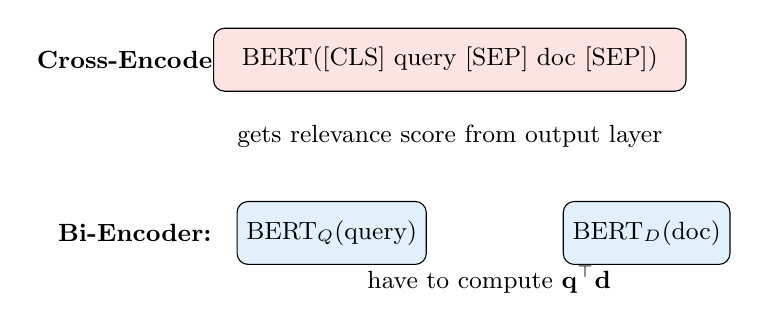
\begin{tikzpicture}[
    box/.style={draw, rounded corners, minimum height=0.8cm, minimum width=2cm, align=center, font=\small},
    arr/.style={-{Stealth[length=2mm]}, thick}
]
% Cross-encoder
\node[font=\small\bfseries] at (-0.5, 2.5) {Cross-Encoder:};
\node[box, fill=dense!15, minimum width=6cm] (ce) at (3.5, 2.5) {BERT([CLS] query [SEP] doc [SEP])};
\node[below=0.3cm of ce, font=\small] {gets relevance score from output layer};

% Bi-encoder
\node[font=\small\bfseries] at (-0.5, 0.3) {Bi-Encoder:};
\node[box, fill=sparse!15] (bq) at (2, 0.3) {$\text{BERT}_Q$(query)};
\node[box, fill=sparse!15] (bd) at (6, 0.3) {$\text{BERT}_D$(doc)};
\node[below=0.3cm of $(bq)!0.5!(bd)$, font=\small] {have to compute $\vq^\top \vd$};
\end{tikzpicture}
\end{center}

\begin{exampleblock}{Key Question}
How do we \textbf{train} the bi-encoder so the dot product captures relevance?
\end{exampleblock}
\end{frame}

\begin{frame}{Cross-Encoder vs.\ Bi-Encoder: Comparison}
\begin{table}
\centering
\footnotesize
\begin{tabular}{lcc}
\toprule
& \textbf{Cross-Encoder} & \textbf{Bi-Encoder} \\
\midrule
Query-doc interaction & Full (all layers) & None (dot product only) \\
Pre-compute doc embeddings & \textcolor{red}{\ding{55}} No & \textcolor{green}{\checkmark} Yes (offline) \\
Use for retrieval & \textcolor{red}{\ding{55}} No (too slow) & \textcolor{green}{\checkmark} Yes (with ANN) \\
Accuracy & Higher & Lower \\
Speed at inference & $\sim$5 ms/pair & $\sim$15 ms total \\
\bottomrule
\end{tabular}
\end{table}
\end{frame}

% ====================================================================
\section{Contrastive Learning for Retrieval}
% ====================================================================

\begin{frame}[plain]
\sectionpage
\end{frame}

\begin{frame}[shrink=15]{Contrastive Learning: Core Principle}
\begin{block}{Objective}
Learn embeddings such that:
$$\text{score}(\vq, \vd^+) \;\gg\; \text{score}(\vq, \vd^-)$$
for relevant pair $(\vq, \vd^+)$ and irrelevant pair $(\vq, \vd^-)$.
\end{block}

\cpause
\vspace{0.5em}

\textbf{Intuition:} The embedding space is a \textbf{map of meaning}.
\begin{itemize}
    \item ``car problems'' and ``automobile issues'' $\to$ nearby points
    \item ``car problems'' and ``car racing'' $\to$ far apart
\end{itemize}\cpause

% \vspace{0.5em}

% \begin{exampleblock}{Connection to Metric Learning}
% Define distance $d(\vq, \vd) = 1 - \cos(\vq, \vd)$ and require:
% $$d(\vq, \vd^+) + \text{margin} < d(\vq, \vd^-)$$
% This is exactly \textbf{deep metric learning} with a learned encoder.
% \end{exampleblock}
\end{frame}

\begin{frame}[shrink=20]{InfoNCE: Noise Contrastive Estimation --- The Classification View}
\begin{center}
% InfoNCE as Classification
% Flow (top→bottom): Query → Documents → Similarity → Softmax → Scores
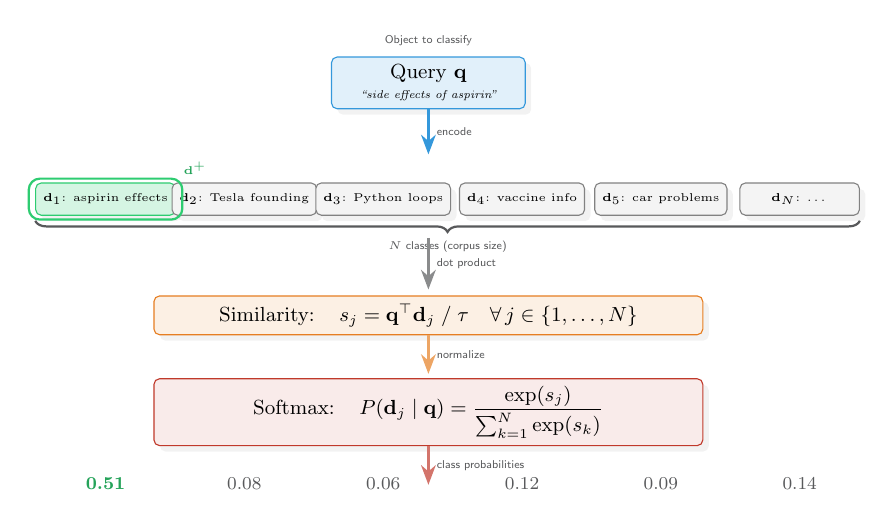
\begin{tikzpicture}[
    scale=0.82, transform shape,
    box/.style={draw, rounded corners=2pt, minimum height=0.6cm, align=center, font=\small, drop shadow={opacity=0.1}},
    arr/.style={-{Stealth[length=2.5mm]}, thick},
]

% --- Row 1: Query (object to classify) ---
\node[box, fill=irSparse!15, draw=irSparse, minimum width=3cm, minimum height=0.8cm] (query) at (5, 0) {Query $\vq$\\[-2pt]\tiny\itshape ``side effects of aspirin''};
\node[font=\tiny\sffamily, text=irInfra, above=0.05cm of query] {Object to classify};

% Arrow from query down to document row
\draw[arr, draw=irSparse] (query.south) -- ++(0, -0.7)
    node[midway, right, font=\tiny\sffamily, text=irInfra] {encode};

% --- Row 2: Document corpus (N classes) ---
\foreach \i/\label/\rel in {
    1/{$\vd_1$: aspirin effects}/1,
    2/{$\vd_2$: Tesla founding}/0,
    3/{$\vd_3$: Python loops}/0,
    4/{$\vd_4$: vaccine info}/0,
    5/{$\vd_5$: car problems}/0,
    6/{$\vd_N$: \ldots}/0
}{
    \pgfmathsetmacro{\xpos}{(\i-1)*2.15}
    \ifnum\rel=1
        \node[box, fill=irHybrid!20, draw=irHybrid, minimum width=1.85cm, font=\tiny, minimum height=0.5cm] (d\i) at (\xpos, -1.8) {\label};
    \else
        \node[box, fill=irMuted!30, draw=irMuted!60!black, minimum width=1.85cm, font=\tiny, minimum height=0.5cm] (d\i) at (\xpos, -1.8) {\label};
    \fi
}

% Positive doc annotation
\draw[irHybrid, thick, rounded corners] ([xshift=-0.1cm, yshift=-0.06cm]d1.south west) rectangle ([xshift=0.1cm, yshift=0.06cm]d1.north east);
\node[font=\tiny\bfseries, text=irHybrid!80!black, anchor=south west] at (d1.north east) {$\vd^+$};

% N classes brace
\draw[decorate, decoration={brace, amplitude=4pt, mirror}, irInfra, thick]
    ([yshift=-0.08cm]d1.south west) -- ([yshift=-0.08cm]d6.south east)
    node[midway, below=5pt, font=\tiny\sffamily, text=irInfra] {$N$ classes (corpus size)};

% Arrow from document row to similarity
\draw[arr, draw=irInfra!70] (5, -2.4) -- (5, -3.2)
    node[midway, right, font=\tiny\sffamily, text=irInfra] {dot product};

% --- Row 3: Similarity layer ---
\node[box, fill=irDense!12, draw=irDense, minimum width=8.5cm, minimum height=0.6cm] (sim) at (5, -3.6)
     {Similarity: \; $s_j = \vq^\top \vd_j \;/\; \tau \quad \forall\, j \in \{1,\ldots,N\}$};

% Arrow from similarity to softmax
\draw[arr, draw=irDense!70] (sim.south) -- ++(0, -0.6)
    node[midway, right, font=\tiny\sffamily, text=irInfra] {normalize};

% --- Row 4: Softmax layer ---
\node[box, fill=irRerank!10, draw=irRerank, minimum width=8.5cm, minimum height=0.6cm] (softmax) at (5, -5.1)
     {Softmax: \; $P(\vd_j \mid \vq) = \dfrac{\exp(s_j)}{\sum_{k=1}^{N} \exp(s_k)}$};

% Arrow from softmax to scores
\draw[arr, draw=irRerank!70] (softmax.south) -- ++(0, -0.6)
    node[midway, right, font=\tiny\sffamily, text=irInfra] {class probabilities};

% --- Row 5: Probability outputs ---
\foreach \i/\prob/\rel in {1/\textbf{0.51}/1, 2/0.08/0, 3/0.06/0, 4/0.12/0, 5/0.09/0, 6/0.14/0}{
    \pgfmathsetmacro{\xpos}{(\i-1)*2.15}
    \ifnum\rel=1
        \node[font=\footnotesize\bfseries, text=irHybrid!80!black] (p\i) at (\xpos, -6.2) {\prob};
    \else
        \node[font=\footnotesize, text=irInfra] (p\i) at (\xpos, -6.2) {\prob};
    \fi
}

\end{tikzpicture}

\end{center}

\begin{exampleblock}{Key Insight}
InfoNCE frames retrieval as \textbf{$N$-way classification}: given query $\vq$, classify which of the $N$ documents in the corpus is the relevant one, using dot-product similarity as the logit.
\end{exampleblock}
\end{frame}

\begin{frame}{Theoretical InfoNCE: The Global View}
\begin{block}{The Goal: Contrastive Estimation}
Given query $\vq$ and its relevant document $\vd^+$, we want to maximize the probability:
$$P(\vd^+ | \vq) = \frac{\exp(\vq^\top \vd^+ / \tau)}{\sum_{\vd \in \mathcal{D}} \exp(\vq^\top \vd / \tau)}$$
where $\mathcal{D}$ is the \textbf{entire corpus} (e.g., 8.8M passages).
\end{block}

\cpause

\begin{block}{The InfoNCE Loss}
The loss minimizes the negative log-probability of the positive document:
$$\mathcal{L}_{\text{InfoNCE}} = -\log P(\vd^+ | \vq) = -\log \frac{\exp(\vq^\top \vd^+ / \tau)}{\sum_{\vd \in \mathcal{D}} \exp(\vq^\top \vd / \tau)}$$
\end{block}

\cpause
\vspace{0.5em}

\end{frame}


\begin{frame}{InfoNCE: The Computational Bottleneck}

\begin{block}{The InfoNCE Loss}
The loss minimizes the negative log-probability of the positive document:
$$\mathcal{L}_{\text{InfoNCE}} = -\log P(\vd^+ | \vq) = -\log \frac{\exp(\vq^\top \vd^+ / \tau)}{\sum_{\vd \in \mathcal{D}} \exp(\vq^\top \vd / \tau)}$$
\end{block}

\cpause
\vspace{0.5em}

\begin{alertblock}{The Computational Bottleneck}
The denominator requires computing the dot product for \textbf{every single document} in the corpus for every gradient step. 
\begin{itemize}
    \item 8.8M documents $\times$ 128 queries per batch $\approx$ 1.1 Billion dot products.
    \item Numerically and computationally \textbf{impossible} to do directly.
\end{itemize}
\end{alertblock}
\end{frame}


\begin{frame}[shrink=10]{The InfoNCE Loss: Practical Approximation}
\begin{block}{In-Batch Contrastive Loss}
We approximate the global sum with a sum over the current \textbf{training batch} of size $B$:
$$\mathcal{L} = -\log \frac{\exp\!\bigl(\vq_i^\top \vp_i^+ / \tau\bigr)}{\displaystyle\sum_{j=1}^{B} \exp\!\bigl(\vq_i^\top \vp_j / \tau\bigr)}$$
\end{block}

\cpause
\vspace{0.3em}

\textbf{Key components:}
\begin{itemize}
    \item $B$: batch size --- provides $B-1$ \textbf{free} negatives per query
    \item $\tau$: temperature --- controls sharpness of the softmax
\end{itemize}
\end{frame}

\begin{frame}[shrink=20]{InfoNCE: From $N$ Classes to $B$ Classes}
\begin{center}
% InfoNCE Batch Approximation: N classes → B classes
% Shows how the full corpus classification is approximated by batch classification
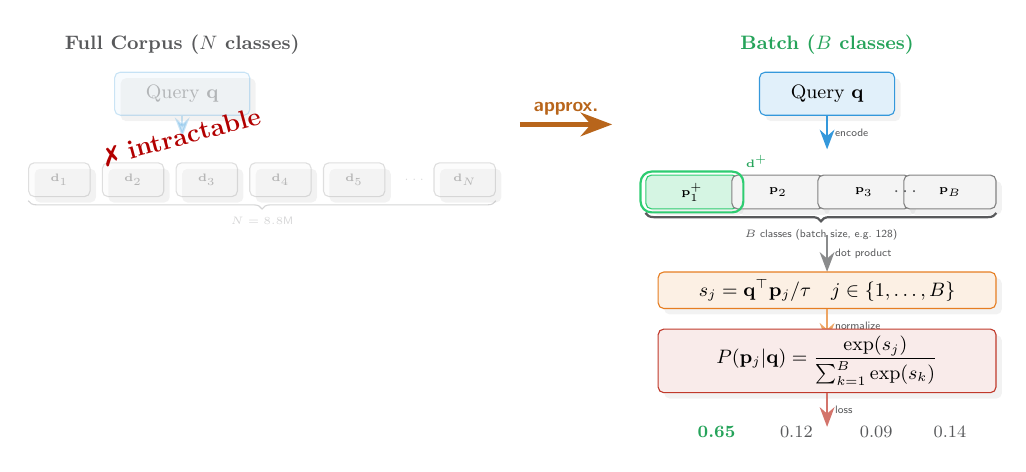
\begin{tikzpicture}[
    scale=0.78, transform shape,
    box/.style={draw, rounded corners=2pt, minimum height=0.55cm, align=center, font=\small, drop shadow={opacity=0.1}},
    arr/.style={-{Stealth[length=2.5mm]}, thick},
    faded/.style={opacity=0.25},
]

% ===== LEFT SIDE: Full corpus (N classes, faded) =====
\node[font=\small\bfseries, text=irInfra] at (-1.5, 0.8) {Full Corpus ($N$ classes)};

% Query
\node[box, fill=irSparse!15, draw=irSparse, minimum width=2.2cm, minimum height=0.7cm, faded] (qL) at (-1.5, 0) {Query $\vq$};

% Documents (faded, compact)
\foreach \i/\xoff in {1/-3.5, 2/-2.3, 3/-1.1, 4/0.1, 5/1.3}{
    \node[box, fill=irMuted!30, draw=irMuted!60!black, minimum width=1cm, font=\tiny, faded] (dL\i) at (\xoff, -1.4) {$\vd_{\i}$};
}
\node[font=\tiny, faded, text=irInfra] at (2.3, -1.4) {$\cdots$};
\node[box, fill=irMuted!30, draw=irMuted!60!black, minimum width=1cm, font=\tiny, faded] (dLN) at (3.1, -1.4) {$\vd_N$};

\draw[arr, draw=irSparse, faded] (qL.south) -- ++(0, -0.35);

% Brace
\draw[decorate, decoration={brace, amplitude=3pt, mirror}, irInfra, faded]
    ([yshift=-0.06cm]dL1.south west) -- ([yshift=-0.06cm]dLN.south east)
    node[midway, below=4pt, font=\tiny\sffamily, text=irInfra, faded] {$N = 8.8$M};

% Crossed out / intractable label
\node[font=\large\bfseries, text=red!70!black, rotate=15] at (-1.5, -0.7) {\ding{55} intractable};

% ===== BIG ARROW =====
\draw[-{Stealth[length=4mm]}, ultra thick, draw=irDense!80!black] (4.0, -0.5) -- (5.5, -0.5)
    node[midway, above, font=\small\sffamily\bfseries, text=irDense!80!black] {approx.};

% ===== RIGHT SIDE: Batch (B classes) =====
\node[font=\small\bfseries, text=irHybrid!80!black] at (9, 0.8) {Batch ($B$ classes)};

% Query
\node[box, fill=irSparse!15, draw=irSparse, minimum width=2.2cm, minimum height=0.7cm] (qR) at (9, 0) {Query $\vq$};

\draw[arr, draw=irSparse] (qR.south) -- ++(0, -0.55)
    node[midway, right, font=\tiny\sffamily, text=irInfra] {encode};

% Documents (batch, fewer, vivid)
\node[box, fill=irHybrid!20, draw=irHybrid, minimum width=1.5cm, font=\tiny] (dR1) at (6.8, -1.6) {$\vp_1^+$};
\node[box, fill=irMuted!30, draw=irMuted!60!black, minimum width=1.5cm, font=\tiny] (dR2) at (8.2, -1.6) {$\vp_2$};
\node[box, fill=irMuted!30, draw=irMuted!60!black, minimum width=1.5cm, font=\tiny] (dR3) at (9.6, -1.6) {$\vp_3$};
\node[box, fill=irMuted!30, draw=irMuted!60!black, minimum width=1.5cm, font=\tiny] (dR4) at (11.0, -1.6) {$\vp_B$};

% Positive doc highlight
\draw[irHybrid, thick, rounded corners] ([xshift=-0.08cm, yshift=-0.05cm]dR1.south west) rectangle ([xshift=0.08cm, yshift=0.05cm]dR1.north east);
\node[font=\tiny\bfseries, text=irHybrid!80!black, anchor=south west] at (dR1.north east) {$\vd^+$};

% ellipsis between p3 and pB
\node[font=\small, text=irInfra] at (10.3, -1.6) {$\cdots$};

% Brace
\draw[decorate, decoration={brace, amplitude=3pt, mirror}, irInfra, thick]
    ([yshift=-0.06cm]dR1.south west) -- ([yshift=-0.06cm]dR4.south east)
    node[midway, below=4pt, font=\tiny\sffamily, text=irInfra] {$B$ classes (batch size, e.g.\ 128)};

% Arrow to similarity
\draw[arr, draw=irInfra!70] (9, -2.3) -- (9, -2.9)
    node[midway, right, font=\tiny\sffamily, text=irInfra] {dot product};

% Similarity
\node[box, fill=irDense!12, draw=irDense, minimum width=5.5cm, minimum height=0.55cm] (simR) at (9, -3.2)
     {$s_j = \vq^\top \vp_j / \tau \quad j \in \{1,\ldots,B\}$};

% Arrow to softmax
\draw[arr, draw=irDense!70] (simR.south) -- ++(0, -0.55)
    node[midway, right, font=\tiny\sffamily, text=irInfra] {normalize};

% Softmax
\node[box, fill=irRerank!10, draw=irRerank, minimum width=5.5cm, minimum height=0.55cm] (softR) at (9, -4.35)
     {$P(\vp_j | \vq) = \dfrac{\exp(s_j)}{\sum_{k=1}^{B} \exp(s_k)}$};

% Arrow to scores
\draw[arr, draw=irRerank!70] (softR.south) -- ++(0, -0.55)
    node[midway, right, font=\tiny\sffamily, text=irInfra] {loss};

% Scores
\node[font=\footnotesize\bfseries, text=irHybrid!80!black] at (7.2, -5.5) {\textbf{0.65}};
\node[font=\footnotesize, text=irInfra] at (8.5, -5.5) {0.12};
\node[font=\footnotesize, text=irInfra] at (9.8, -5.5) {0.09};
\node[font=\footnotesize, text=irInfra] at (11.0, -5.5) {0.14};

\end{tikzpicture}

\end{center}

\begin{exampleblock}{Batch Approximation}
Instead of classifying over the \textbf{entire corpus} ($N$ classes), we classify over only the \textbf{batch} ($B$ classes). Each batch provides $B{-}1$ in-batch negatives for free.
\end{exampleblock}
\end{frame}


% ====================================================================
\section{Dense Passage Retrieval (DPR)}
% ====================================================================

\begin{frame}[plain]
\sectionpage
\end{frame}

\begin{frame}{DPR: Architecture (Karpukhin et al., 2020)}
\begin{center}
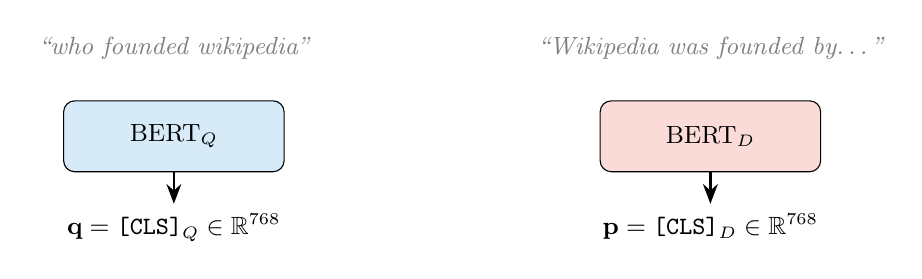
\begin{tikzpicture}[
    box/.style={draw, rounded corners, minimum height=0.9cm, minimum width=2.8cm, align=center, font=\small},
    arr/.style={-{Stealth[length=2.5mm]}, thick}
]
\node[box, fill=sparse!20] (bertq) {$\text{BERT}_Q$};
\node[box, fill=dense!20, right=4cm of bertq] (bertd) {$\text{BERT}_D$};
\node[below=0.4cm of bertq, font=\small] (clsq) {$\vq = \texttt{[CLS]}_Q \in \mathbb{R}^{768}$};
\node[below=0.4cm of bertd, font=\small] (clsd) {$\vp = \texttt{[CLS]}_D \in \mathbb{R}^{768}$};
\node[above=0.4cm of bertq, font=\small\itshape, text=gray] {``who founded wikipedia''};
\node[above=0.4cm of bertd, font=\small\itshape, text=gray] {``Wikipedia was founded by\ldots''};

\draw[arr] (bertq) -- (clsq);
\draw[arr] (bertd) -- (clsd);
\end{tikzpicture}
\end{center}

\vspace{0.5em}

\begin{block}{Key Design Choices}
\begin{itemize}
    % \item \textbf{Separate encoders:} $\text{BERT}_Q \neq \text{BERT}_D$ (different weights, can specialize)
    \item \textbf{Representation:} \texttt{[CLS]} token output --- single vector per text
    \item \textbf{Similarity:} $\text{score}(\vq, \vp) = \vq^\top \vp$ (dot product)
    % \item \textbf{No interaction:} Query and passage never ``see'' each other during encoding
\end{itemize}
\end{block}
\end{frame}

\begin{frame}{DPR: Training Recipe --- Loss \& Negatives}
\textbf{Loss:} InfoNCE with in-batch negatives
$$\mathcal{L} = -\log \frac{e^{\vq_i^\top \vp_i^+/\tau}}{\sum_{j=1}^{B} e^{\vq_i^\top \vp_j / \tau}}$$

\vspace{0.8em}

\textbf{Negatives per query:}
\begin{enumerate}
    \item $B-1$ in-batch negatives (free!)
    \item 1 BM25 hard negative (precomputed)
\end{enumerate}

\vspace{1em}

\begin{exampleblock}{Key Insight}
Mixing \textbf{one} BM25 hard negative with in-batch random negatives is surprisingly effective. The BM25 negative is lexically similar but not relevant --- forces the model beyond surface matching.
\end{exampleblock}
\end{frame}


\begin{frame}{DPR: Why BM25 Hard Negatives?}
\textbf{Query:} ``side effects of aspirin''

\vspace{1em}

\textbf{Random negative:} ``The capital of France is Paris\ldots''
\begin{itemize}
    \item $\vq^\top \vd^- \approx 0.05$ --- trivially easy, \textbf{no learning signal}
\end{itemize}\cpause

\cpause
\vspace{0.5em}

\textbf{BM25 hard negative:} ``Aspirin was invented by Bayer in 1899\ldots''
\begin{itemize}
    \item Contains ``aspirin'' $\to$ BM25 ranks it high
    \item But \textbf{not about side effects} $\to$ not relevant
    \item $\vq^\top \vd^- \approx 0.6$ --- confusing, \textbf{strong learning signal!}
\end{itemize}\cpause

\cpause
\vspace{1em}

\begin{alertblock}{The Principle}
The model must learn: ``just because a passage mentions aspirin doesn't mean it's about side effects.'' This is \textbf{exactly} what BM25 cannot do.
\end{alertblock}
\end{frame}

\begin{frame}{DPR: Results \& Significance}
\begin{center}
\begin{tabular}{lccc}
\toprule
\textbf{Method} & \textbf{NQ Top-20 Recall} & \textbf{MS MARCO MRR@10} & \textbf{Params} \\
\midrule
BM25 & 59.1 & 18.7 & --- \\
\textbf{DPR} & \textbf{78.4} & \textbf{31.1} & 220M \\
\bottomrule
\end{tabular}
\end{center}

\vspace{0.5em}

\begin{block}{Why DPR Matters}
\begin{itemize}
    \item First system to conclusively show \textbf{dense $>$ sparse} for open-domain QA
    \item +19pp top-20 recall over BM25 on Natural Questions
    \item Enabled the modern ``retriever + reader'' paradigm
\end{itemize}\cpause
\end{block}

\cpause
\vspace{0.5em}

\begin{alertblock}{But\ldots}
A single 768-dim vector for the entire document? That's a severe \textbf{information bottleneck}. Can we do better?
\end{alertblock}
\end{frame}

% ====================================================================
\section{ColBERT: Late Interaction}
% ====================================================================

\begin{frame}[plain]
\sectionpage
\end{frame}

\begin{frame}[shrink=10]{The Single-Vector Bottleneck}
\begin{alertblock}{Problem with DPR}
The \textbf{entire} document is compressed into a single 768-dim vector.
\end{alertblock}

\vspace{0.5em}

\begin{center}
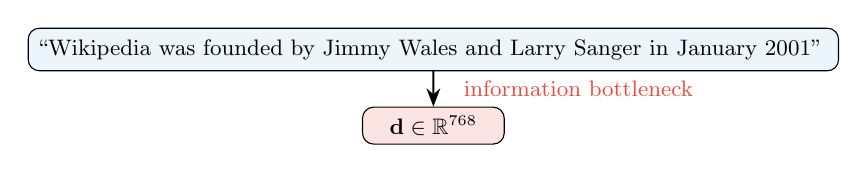
\begin{tikzpicture}[font=\small, scale=0.9, transform shape]
\node[draw, fill=sparse!10, rounded corners, minimum width=9cm, minimum height=0.6cm, align=center] (doc) {
    ``Wikipedia was founded by Jimmy Wales and Larry Sanger in January 2001''
};
\node[draw, fill=dense!15, rounded corners, minimum width=2cm, below=0.5cm of doc] (vec) {$\vd \in \mathbb{R}^{768}$};
\draw[-{Stealth}, thick] (doc) -- (vec) node[midway, right, xshift=0.3cm] {\textcolor{dense}{information bottleneck}};
\end{tikzpicture}
\end{center}

\cpause
\vspace{0.2em}

\textbf{Consequences:}
\begin{itemize}
    \item Cannot capture fine-grained token-level alignments
    \item ``\textbf{Who} founded Wikipedia?'' vs.\ ``\textbf{When} was Wikipedia founded?'' $\to$ similar scores!
    \item Long documents lose information
\end{itemize}\cpause

\vspace{0.2em}

\begin{exampleblock}{Solution}
Keep \textbf{all} token embeddings, not just \texttt{[CLS]}. Compare at the token level.
\end{exampleblock}
\end{frame}

\begin{frame}[fragile]{ColBERT: Architecture (Khattab \& Zaharia, 2020)}
\begin{block}{Key Idea}
Encode query and document \textbf{separately} (like bi-encoder), but compare at the \textbf{token level} using MaxSim.
\end{block}

\vspace{0.2em}

\begin{center}
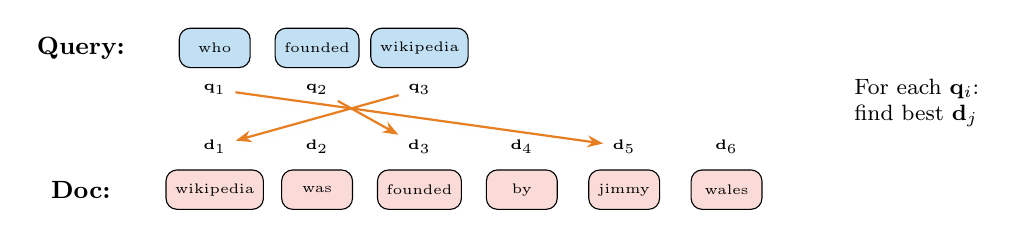
\begin{tikzpicture}[
    tok/.style={draw, rounded corners, fill=#1, minimum width=0.9cm, minimum height=0.5cm, font=\tiny},
    arr/.style={-{Stealth[length=2mm]}, thin, gray}
]
% Query tokens
\node[font=\small\bfseries] at (-1.2, 1.8) {Query:};
\foreach \i/\w/\c in {0/who/sparse!30, 1/founded/sparse!30, 2/wikipedia/sparse!30} {
    \node[tok=\c] (q\i) at (1.3*\i + 0.5, 1.8) {\w};
    \node[font=\tiny, below=0.08cm of q\i] (qe\i) {$\vq_{\the\numexpr\i+1}$};
}

% Doc tokens
\node[font=\small\bfseries] at (-1.2, 0) {Doc:};
\foreach \i/\w/\c in {0/wikipedia/dense!20, 1/was/dense!20, 2/founded/dense!20, 3/by/dense!20, 4/jimmy/dense!20, 5/wales/dense!20} {
    \node[tok=\c] (d\i) at (1.3*\i + 0.5, 0) {\w};
    \node[font=\tiny, above=0.08cm of d\i] (de\i) {$\vd_{\the\numexpr\i+1}$};
}

% MaxSim arrows (best matches)
\draw[arr, thick, dense] (qe0) -- (de4);
\draw[arr, thick, dense] (qe1) -- (de2);
\draw[arr, thick, dense] (qe2) -- (de0);

\node[font=\footnotesize, anchor=west, align=left] at (8.5, 1.1) {For each $\vq_i$:\\find best $\vd_j$};
\end{tikzpicture}
\end{center}

\cpause
\vspace{0.3em}

\begin{exampleblock}{Late Interaction}
Documents are encoded \textbf{offline} (token-level embeddings stored). The ``interaction'' happens \textbf{late} --- only at query time via MaxSim.
\end{exampleblock}
\end{frame}

\begin{frame}[shrink=10]{ColBERT: MaxSim Scoring}
\begin{block}{MaxSim Definition}
$$\text{MaxSim}(\vq, \vd) = \sum_{i=1}^{|\vq|} \max_{j=1}^{|\vd|}\; \cos(\vq_i, \vd_j)$$
\end{block}

\vspace{0.3em}

\textbf{Step by step:}
\begin{enumerate}
    \item For each query token $\vq_i$, find the document token $\vd_j$ with highest cosine similarity
    \item Take that maximum similarity
    \item Sum across all query tokens
\end{enumerate}

\cpause
\vspace{0.5em}

\textbf{Properties:}
\begin{itemize}
    \item \textbf{Asymmetric:} Every query token must find a match; document tokens can be ignored
    \item \textbf{Decomposable:} Document embeddings precomputed and stored offline
    \item Token embeddings: $\vq_i, \vd_j \in \mathbb{R}^{128}$ (projected down from 768)
\end{itemize}
\end{frame}

\begin{frame}[shrink=10]{Worked Example: MaxSim Scoring}
\textbf{Query:} ``who founded wikipedia'' (3 tokens)\\
\textbf{Document:} ``wikipedia was founded by jimmy wales'' (6 tokens)

\vspace{0.5em}

\begin{table}
\centering
\footnotesize
\begin{tabular}{lcccccc}
\toprule
& \textit{wikipedia} & \textit{was} & \textit{founded} & \textit{by} & \textit{jimmy} & \textit{wales} \\
\midrule
\textit{who}       & 0.12 & 0.08 & 0.15 & 0.10 & \textbf{0.72} & 0.45 \\
\textit{founded}   & 0.20 & 0.05 & \textbf{0.95} & 0.10 & 0.12 & 0.08 \\
\textit{wikipedia} & \textbf{0.98} & 0.06 & 0.18 & 0.04 & 0.10 & 0.15 \\
\bottomrule
\end{tabular}
\end{table}

\cpause
\vspace{0.5em}

$$\text{MaxSim} = \underbrace{0.72}_{\text{who}\to\text{jimmy}} + \underbrace{0.95}_{\text{founded}\to\text{founded}} + \underbrace{0.98}_{\text{wikipedia}\to\text{wikipedia}} = \mathbf{2.65}$$

\vspace{0.5em}

\begin{exampleblock}{Notice}
``who'' aligns with ``jimmy'' (the answer entity) --- the model learns \textbf{semantic alignment}, not just exact matching.
\end{exampleblock}
\end{frame}

\begin{frame}{ColBERT: Efficiency vs.\ Accuracy}
\begin{table}
\centering
\small
\begin{tabular}{lccc}
\toprule
& \textbf{DPR (Bi-Enc)} & \textbf{ColBERT} & \textbf{Cross-Encoder} \\
\midrule
Interaction & None (dot prod) & Late (MaxSim) & Full (cross-attn) \\
Pre-compute docs & \textcolor{green}{\checkmark} (1 vec) & \textcolor{green}{\checkmark} ($n$ vecs) & \textcolor{red}{\ding{55}} \\
Use for retrieval & \textcolor{green}{\checkmark} With ANN & \textcolor{green}{\checkmark} With ANN & \textcolor{red}{\ding{55}} Too slow \\
Speedup vs.\ CE & $\sim$1000$\times$ & $\sim$100$\times$ & $1\times$ \\
MS MARCO MRR@10 & 31.1 & 36.0 & 39.0 \\
Storage per doc & $768 \times 4$B = 3 KB & $128 \times 128 \times 4$B $\approx$ 64 KB & N/A \\
\bottomrule
\end{tabular}
\end{table}

\cpause
\vspace{0.5em}

\begin{exampleblock}{Sweet Spot}
ColBERT gives near-cross-encoder accuracy at bi-encoder-like speed. Trade-off: \textbf{much higher storage} (one vector per token, not per document).
\end{exampleblock}
\end{frame}

% ====================================================================
\section{Hard Negatives Mining}
% ====================================================================
\begin{frame}[plain]
\sectionpage
\end{frame}


\begin{frame}[shrink=15]{Hard vs.\ Easy Negatives: Why It Matters}
\begin{center}
% Hard vs Easy Negatives Visualization
% Left: scatter plot with positives, hard negatives, easy negatives, decision boundaries
% Right: InfoNCE formula with highlighted negative sum
\begin{tikzpicture}[
    scale=0.78, transform shape,
    arr/.style={-{Stealth[length=2.5mm]}, thick},
]

% ===== LEFT: Scatter Plot =====
% Axes
\draw[arr, irInfra!60] (-0.3, -0.3) -- (7.5, -0.3);
\draw[arr, irInfra!60] (-0.3, -0.3) -- (-0.3, 6.2);

% --- Positives (green cluster, top-left) ---
\foreach \x/\y in {1.0/4.8, 1.5/5.2, 0.8/5.5, 1.8/4.5, 1.3/5.0, 2.0/5.3, 0.6/4.6}{
    \fill[irHybrid!80!black] (\x, \y) circle (4pt);
}

% --- Hard negatives (dark red, close to positives) ---
\foreach \x/\y in {2.5/4.0, 3.0/4.5, 2.2/3.7, 2.8/3.5, 3.3/4.2}{
    \fill[irRerank!90!black] (\x, \y) circle (4pt);
}

% --- Easy negatives (lighter red, far from positives — bottom-right) ---
\foreach \x/\y in {5.0/1.0, 5.5/0.8, 6.0/1.3, 5.2/0.5, 5.8/1.6, 6.3/0.9, 5.5/1.8, 6.5/1.5, 5.0/1.8, 6.0/0.4, 5.7/2.1}{
    \fill[red!50!orange] (\x, \y) circle (4pt);
}

% --- Decision boundary: Weak classifier (easy negatives only) ---
\draw[red!50!orange, thick, dashed, line width=1.2pt]
    plot[smooth] coordinates {(3.5, 6.2) (3.7, 4.0) (4.0, 2.5) (4.2, 0.5) (4.3, -0.3)};
\node[font=\tiny\sffamily, text=red!50!orange, rotate=-82, anchor=south] at (4.4, 3.5) {weak boundary};

% --- Decision boundary: Strong classifier (hard negatives) ---
\draw[irHybrid!80!black, thick, line width=1.5pt]
    plot[smooth] coordinates {(1.5, 6.2) (1.8, 5.0) (2.2, 4.2) (2.4, 3.2) (2.5, 2.0) (2.4, 0.5) (2.3, -0.3)};
\node[font=\tiny\sffamily\bfseries, text=irHybrid!80!black, rotate=-85, anchor=south] at (1.8, 3.0) {strong boundary};

% ===== LEGEND (bottom-left) =====
\node[anchor=north west] at (-0.2, -0.8) {
    \begin{tikzpicture}[font=\footnotesize]
        \fill[irHybrid!80!black] (0, 0) circle (3.5pt);
        \node[anchor=west] at (0.25, 0) {Positives ($\vd^+$)};
        \fill[irRerank!90!black] (0, -0.45) circle (3.5pt);
        \node[anchor=west] at (0.25, -0.45) {Hard negatives};
        \fill[red!50!orange] (0, -0.9) circle (3.5pt);
        \node[anchor=west] at (0.25, -0.9) {Easy negatives};
    \end{tikzpicture}
};

% ===== RIGHT: Loss Formula =====
\node[anchor=north west, font=\small] at (8.5, 6.0) {
\begin{minipage}{5.5cm}
\textbf{InfoNCE Loss:}
\vspace{0.3em}

$\mathcal{L}(\vq_i, \vp_i^+, \vp_{i,1}^-, \cdots, \vp_{i,n}^-)$

\vspace{0.5em}

$= -\log \dfrac{e^{\text{sim}(\vq_i, \vp_i^+)}}{e^{\text{sim}(\vq_i, \vp_i^+)} + \tikz[baseline=(X.base)]{\node[fill=yellow!40, rounded corners=2pt, inner sep=3pt] (X) {$\displaystyle\sum_{j=1}^{n} e^{\text{sim}(\vq_i, \vp_{i,j}^-)}$};}}$

\vspace{0.8em}

\textcolor{irRerank!80!black}{\textbf{Hard negatives}} are close to the positives in embedding space $\to$ large $\text{sim}(\vq, \vp^-)$.

\vspace{0.3em}

This makes the \tikz[baseline=(Y.base)]{\node[fill=yellow!40, rounded corners=2pt, inner sep=2pt, font=\small] (Y) {denominator};} large, the loss \textbf{harder to minimize}, and gradients \textbf{more informative}.
\end{minipage}
};

\end{tikzpicture}

\end{center}
\end{frame}

\begin{frame}{The Evolving Encoder and Negative Quality}
\begin{block}{Key Insight: What Counts as ``Hard'' Changes Over Training}
The encoder's understanding of relevance \textbf{evolves} across training epochs. This changes which negatives are informative:
\end{block}

\cpause
\vspace{0.5em}

\textbf{Early training:} The encoder has no notion of relevance.
\begin{itemize}
    \item BM25 negatives (lexically similar but irrelevant) are \textbf{not yet hard} --- the model cannot even distinguish basic relevance.
    \item Random negatives provide sufficient learning signal.
\end{itemize}

\cpause
\vspace{0.5em}

\textbf{Later training:} The encoder understands basic relevance.
\begin{itemize}
    \item Random negatives become \textbf{trivially easy} --- zero gradient.
    \item BM25 negatives now become \textbf{genuinely hard} --- the model must learn to distinguish lexical overlap from true relevance.
\end{itemize}

% \begin{alertblock}{Implication}
% The optimal negative sampling strategy is \textbf{not fixed} --- it should adapt to the encoder's current capability.
% \end{alertblock}
\end{frame}


\begin{frame}[shrink=15]{The Evolving Encoder: Representations Shift Over Training}
\begin{center}
% Evolving Encoder: Representations change across training epochs
% Three panels showing the same documents at different positions as encoder improves
\begin{tikzpicture}[
    scale=0.75, transform shape,
    arr/.style={-{Stealth[length=2mm]}, thick},
    panel/.style={draw=irInfra!30, rounded corners=3pt, inner sep=5pt},
]

% ===== PANEL 1: Epoch t (early — everything mixed) =====
\begin{scope}[shift={(0,0)}]
    \node[font=\small\bfseries, text=irInfra] at (2.2, 5.2) {Epoch $t$ (early)};

    % Axes
    \draw[arr, irInfra!40] (-0.2, -0.2) -- (4.5, -0.2);
    \draw[arr, irInfra!40] (-0.2, -0.2) -- (-0.2, 4.8);

    % Positives (green — scattered, no clear cluster)
    \foreach \x/\y in {1.2/3.0, 2.5/1.5, 0.8/1.8, 3.2/3.5, 1.8/4.0}{
        \fill[irHybrid!80!black] (\x, \y) circle (3.5pt);
    }

    % Hard negatives (dark red — also scattered, intermixed)
    \foreach \x/\y in {1.5/2.5, 2.8/2.8, 2.0/3.2, 3.0/1.0, 0.5/3.8}{
        \fill[irRerank!90!black] (\x, \y) circle (3.5pt);
    }

    % Easy negatives (orange)
    \foreach \x/\y in {3.5/4.2, 0.6/0.5, 3.8/0.8, 1.0/4.5, 3.0/2.0}{
        \fill[red!50!orange] (\x, \y) circle (3.5pt);
    }

    % No clear boundary — dashed uncertain line
    \draw[irInfra!40, dashed, thin] plot[smooth] coordinates {(0.2, 4.6) (1.5, 2.8) (2.5, 1.5) (4.0, 0.2)};
    \node[font=\tiny\sffamily, text=irInfra!50, anchor=north] at (2.2, -0.5) {no separation};
\end{scope}

% ===== ARROW 1→2 =====
\draw[-{Stealth[length=3mm]}, ultra thick, draw=irDense!70] (5.0, 2.3) -- (5.8, 2.3)
    node[midway, above, font=\tiny\sffamily\bfseries, text=irDense!70] {train};

% ===== PANEL 2: Epoch t+1 (mid — beginning to separate) =====
\begin{scope}[shift={(6.2, 0)}]
    \node[font=\small\bfseries, text=irInfra] at (2.2, 5.2) {Epoch $t{+}1$};

    % Axes
    \draw[arr, irInfra!40] (-0.2, -0.2) -- (4.5, -0.2);
    \draw[arr, irInfra!40] (-0.2, -0.2) -- (-0.2, 4.8);

    % Positives (green — starting to cluster top-left)
    \foreach \x/\y in {0.8/4.2, 1.3/3.8, 0.6/3.5, 1.6/4.5, 1.0/4.0}{
        \fill[irHybrid!80!black] (\x, \y) circle (3.5pt);
    }

    % Hard negatives (dark red — nearby but separating)
    \foreach \x/\y in {2.0/3.2, 2.5/3.8, 1.8/2.8, 2.8/3.0, 2.3/2.5}{
        \fill[irRerank!90!black] (\x, \y) circle (3.5pt);
    }

    % Easy negatives (orange — clearly far away now)
    \foreach \x/\y in {3.5/0.8, 3.8/1.2, 4.0/0.5, 3.2/1.5, 3.6/0.3}{
        \fill[red!50!orange] (\x, \y) circle (3.5pt);
    }

    % Weak boundary (separates easy only)
    \draw[red!50!orange, dashed, thick] plot[smooth] coordinates {(2.8, 4.8) (3.0, 3.0) (3.0, 1.8) (2.8, 0.0)};
    \node[font=\tiny\sffamily, text=red!50!orange, anchor=north] at (2.2, -0.5) {easy separated};
\end{scope}

% ===== ARROW 2→3 =====
\draw[-{Stealth[length=3mm]}, ultra thick, draw=irDense!70] (11.2, 2.3) -- (12.0, 2.3)
    node[midway, above, font=\tiny\sffamily\bfseries, text=irDense!70] {train};

% ===== PANEL 3: Epoch t+2 (late — well separated) =====
\begin{scope}[shift={(12.4, 0)}]
    \node[font=\small\bfseries, text=irInfra] at (2.2, 5.2) {Epoch $t{+}2$ (converged)};

    % Axes
    \draw[arr, irInfra!40] (-0.2, -0.2) -- (4.5, -0.2);
    \draw[arr, irInfra!40] (-0.2, -0.2) -- (-0.2, 4.8);

    % Positives (green — tight cluster top-left)
    \foreach \x/\y in {0.6/4.5, 0.9/4.2, 0.5/4.8, 1.2/4.0, 0.8/4.6}{
        \fill[irHybrid!80!black] (\x, \y) circle (3.5pt);
    }

    % Hard negatives (dark red — separated but still closest)
    \foreach \x/\y in {2.0/3.0, 2.4/2.6, 1.8/2.3, 2.6/2.8, 2.2/3.3}{
        \fill[irRerank!90!black] (\x, \y) circle (3.5pt);
    }

    % Easy negatives (orange — far bottom-right)
    \foreach \x/\y in {3.5/0.5, 3.8/0.8, 4.0/0.3, 3.3/1.0, 3.7/1.2}{
        \fill[red!50!orange] (\x, \y) circle (3.5pt);
    }

    % Strong boundary (separates hard negatives too)
    \draw[irHybrid!80!black, thick, line width=1.3pt] plot[smooth] coordinates {(1.2, 4.8) (1.5, 3.8) (1.6, 3.0) (1.5, 2.0) (1.3, 0.5)};
    \node[font=\tiny\sffamily\bfseries, text=irHybrid!80!black, anchor=north] at (2.2, -0.5) {hard separated};
\end{scope}

% ===== LEGEND =====
\node[anchor=north west] at (0, -1.3) {
    \begin{tikzpicture}[font=\footnotesize]
        \fill[irHybrid!80!black] (0, 0) circle (3pt);
        \node[anchor=west] at (0.22, 0) {Positives ($\vd^+$)};
        \fill[irRerank!90!black] (3.5, 0) circle (3pt);
        \node[anchor=west] at (3.72, 0) {Hard negatives};
        \fill[red!50!orange] (6.8, 0) circle (3pt);
        \node[anchor=west] at (7.02, 0) {Easy negatives};
    \end{tikzpicture}
};

\end{tikzpicture}

\end{center}

\cpause
\vspace{0.3em}

\begin{alertblock}{Implication}
The optimal negative sampling strategy is \textbf{not fixed} --- it should adapt to the encoder's current capability.
\end{alertblock}
\end{frame}


\begin{frame}{From Static to Dynamic Negatives}
\begin{block}{Static Negatives (e.g., BM25)}
Negatives are chosen \textbf{once, before training} and remain fixed:
\begin{itemize}
    \item Cheap to compute (run BM25 once).
    \item Eventually become too easy as the encoder improves.
\end{itemize}
\end{block}

\cpause
\vspace{0.5em}

\begin{exampleblock}{Dynamic Negatives (e.g., ANCE)}
Negatives are defined by the \textbf{current encoder state}:
\begin{itemize}
    \item A \textbf{hard negative} = a document the model \textbf{currently} scores high, but is \textbf{not} the ground-truth relevant document.
    \item These are the most confusing examples \emph{right now} --- maximally informative gradients.
    \item Requires periodically re-encoding the corpus and refreshing the index.
\end{itemize}
\end{exampleblock}

\cpause
\vspace{0.3em}

\begin{center}
\textbf{Static:} fixed before training \quad $\longrightarrow$ \quad \textbf{Dynamic:} adapts with the model
\end{center}
\end{frame}


% \begin{frame}{The Landscape of Negative Sampling}
% \textbf{The Challenge:} The denominator in InfoNCE over $\mathcal{D}$ is the bottleneck. The quality of our approximation depends on the \textbf{negatives} we choose.

% \vspace{1em}

% \begin{itemize}
%     \item \textbf{Random Negatives:} Passages sampled uniformly from the corpus. Usually too easy (e.g., query ``Python'' vs document ``Aspirin'').
%     \item \textbf{In-Batch Negatives:} Using documents from other queries in the same batch. Computationally efficient (``free'').
%     \item \textbf{BM25 Hard Negatives:} Passages that contain query terms but are not relevant. Forces model to learn fine-grained semantics.
%     \item \textbf{Dynamic Hard Negatives (ANCE):} Passages that the model \textbf{currently} thinks are relevant (top predictions). Most effective but requires periodic index refreshes.
% \end{itemize}
% \end{frame}

% \begin{frame}[shrink=5]{The Hard Negative Problem (Xiong et al., 2021)}
% \begin{alertblock}{Observation}
% Most in-batch negatives are \textbf{trivially easy}. The model separates them instantly and stops learning.
% \end{alertblock}

% \vspace{0.5em}

% \begin{center}
% \begin{tikzpicture}[font=\small]
% \draw[-{Stealth}, thick] (0,0) -- (9,0) node[right] {Training steps};
% \draw[-{Stealth}, thick] (0,0) -- (0,3) node[above] {$\|\nabla \mathcal{L}\|$};

% \draw[sparse, thick] plot[smooth] coordinates {(0.5,2.5) (1.5,1.5) (3,0.5) (5,0.2) (7,0.1) (8.5,0.05)};
% \node[sparse, font=\footnotesize, anchor=west] at (6.5,0.4) {Random negatives};

% \draw[dense, thick] plot[smooth] coordinates {(0.5,2.5) (1.5,2.1) (3,1.7) (5,1.2) (7,0.8) (8.5,0.5)};
% \node[dense, font=\footnotesize, anchor=west] at (6.5,2.2) {Hard negatives (ANCE)};
% \end{tikzpicture}
% \end{center}

% \cpause
% \vspace{0.3em}

% Random negatives $\Rightarrow$ gradients vanish early $\Rightarrow$ \textbf{slow convergence}.
% \end{frame}

\begin{frame}[fragile]{ANCE: Asynchronous Index Refresh}
\begin{block}{Core Innovation}
Maintain an ANN index during training. Use the model's \textbf{own} top-$k$ nearest passages as hard negatives.
\end{block}

\vspace{0.5em}

\begin{center}
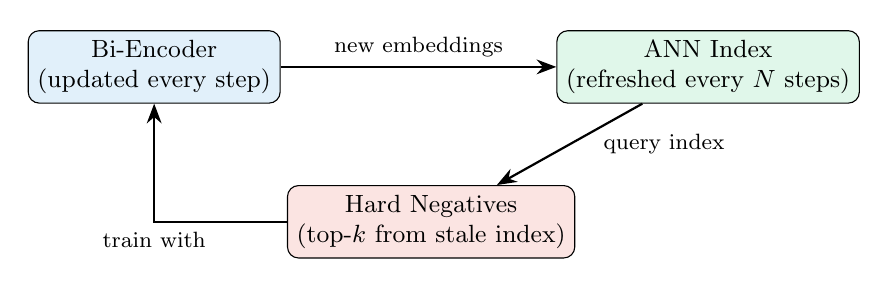
\begin{tikzpicture}[
    box/.style={draw, rounded corners, fill=#1, minimum height=0.8cm, minimum width=2.8cm, align=center, font=\small},
    arr/.style={-{Stealth[length=2.5mm]}, thick}
]
\node[box=sparse!15] (enc) {Bi-Encoder\\(updated every step)};
\node[box=hybrid!15, right=3.5cm of enc] (idx) {ANN Index\\(refreshed every $N$ steps)};
\node[box=dense!15, below=1.5cm of $(enc)!0.5!(idx)$] (neg) {Hard Negatives\\(top-$k$ from stale index)};

\draw[arr] (enc) -- (idx) node[midway, above, font=\footnotesize] {new embeddings};
\draw[arr] (idx) -- (neg) node[midway, right, font=\footnotesize, xshift=0.3cm] {query index};
\draw[arr] (neg) -| (enc) node[midway, below, font=\footnotesize] {train with};
\end{tikzpicture}
\end{center}

\cpause
\vspace{0.3em}

% \begin{exampleblock}{Why the Lag is a Feature}
% The index lags by $N$ steps. Negatives are hard (from a recent model) but not \textbf{impossibly} hard (from the current model). This stabilizes training.
% \end{exampleblock}
\end{frame}



\begin{frame}[shrink=15]{ANCE: Results}
\begin{center}
\begin{tabular}{lccc}
\toprule
\textbf{Method} & \textbf{NQ Top-20 R} & \textbf{MS MARCO MRR@10} & \textbf{Negatives} \\
\midrule
BM25 & 59.1 & 18.7 & --- \\
DPR (BM25 neg.) & 78.4 & 31.1 & Static / lexical \\
\textbf{ANCE} & \textbf{81.9} & \textbf{33.0} & Dynamic / semantic \\
\bottomrule
\end{tabular}
\end{center}

\cpause
\vspace{1em}

\begin{exampleblock}{Key Takeaway}
The \textbf{only} difference between DPR and ANCE is the negative sampling strategy. Semantic hard negatives from the model's own index are strictly better than BM25 hard negatives.
\end{exampleblock}

\begin{alertblock}{Implication}
Negative sampling is a \textbf{first-order concern} in dense retrieval. \\The model and architecture stay the same --- the negatives matter most.
\end{alertblock}
\end{frame}

% ====================================================================
\section{Evaluation \& The Zero-Shot Challenge}
% ====================================================================

\begin{frame}[plain]
\sectionpage
\end{frame}

\begin{frame}{Key Benchmarks}
\begin{table}
\centering
\small
\begin{tabular}{lccl}
\toprule
\textbf{Benchmark} & \textbf{Corpus} & \textbf{Queries} & \textbf{Primary Metric} \\
\midrule
MS MARCO & 8.8M passages & 500K train & MRR@10 \\
Natural Questions & 21M passages & 3.5K test & Top-20 Recall \\
BEIR (18 tasks) & Varies & Varies & nDCG@10 (zero-shot) \\
TREC-DL 2019/20 & 8.8M passages & 43/54 & nDCG@10 \\
\bottomrule
\end{tabular}
\end{table}

\cpause
\vspace{0.5em}

\begin{alertblock}{Critical Distinction}
\begin{itemize}
    \item MS MARCO / NQ: \textbf{In-domain} (train \& test same distribution)
    \item BEIR: \textbf{Zero-shot} (train on MS MARCO, test on 18 diverse tasks)
    \item Dense methods excel in-domain but often struggle on BEIR!
\end{itemize}
\end{alertblock}
\end{frame}

\begin{frame}{The Zero-Shot Challenge: BEIR}
\begin{center}
\begin{tabular}{lccccc}
\toprule
& \textbf{BM25} & \textbf{DPR} & \textbf{ColBERT} & \textbf{ANCE} & \textbf{Contriever} \\
\midrule
BEIR Avg nDCG@10 & 47.3 & 33.2 & 41.5 & 37.7 & 48.5 \\
\bottomrule
\end{tabular}
\end{center}

\vspace{1em}
\cpause

\begin{alertblock}{Surprising Finding}
\textbf{BM25 outperforms} most dense models on zero-shot BEIR!
\end{alertblock}

\textbf{Why?}
\begin{itemize}
    \item Dense models overfit to MS MARCO query structure.
    \item BM25 is distribution-agnostic (just term statistics).
    \item BEIR includes diverse tasks (fact-checking, etc.) where semantic matching isn't always enough.
\end{itemize}
\end{frame}

\begin{frame}{Solving Zero-Shot: Contriever}
\begin{block}{Contriever (Izacard et al., 2022)}
Instead of learning retrieval from \textbf{manual relevance labels},
how can we learn from \textbf{raw text alone} using contrastive learning.
\end{block}

\vspace{1em}
\cpause

\begin{exampleblock}{Result}
Contriever (48.5) finally beats BM25 (47.3) on average across BEIR, showing that domain-agnostic dense retrieval is possible.
\end{exampleblock}
\end{frame}

\begin{frame}[shrink=15]{How Contriever Solves the Zero-Shot Problem}
\begin{center}
% Contriever: Document Views + MoCo Queue Visualization
% Shows: document → random crop → two views → encoder → contrastive loss with queue
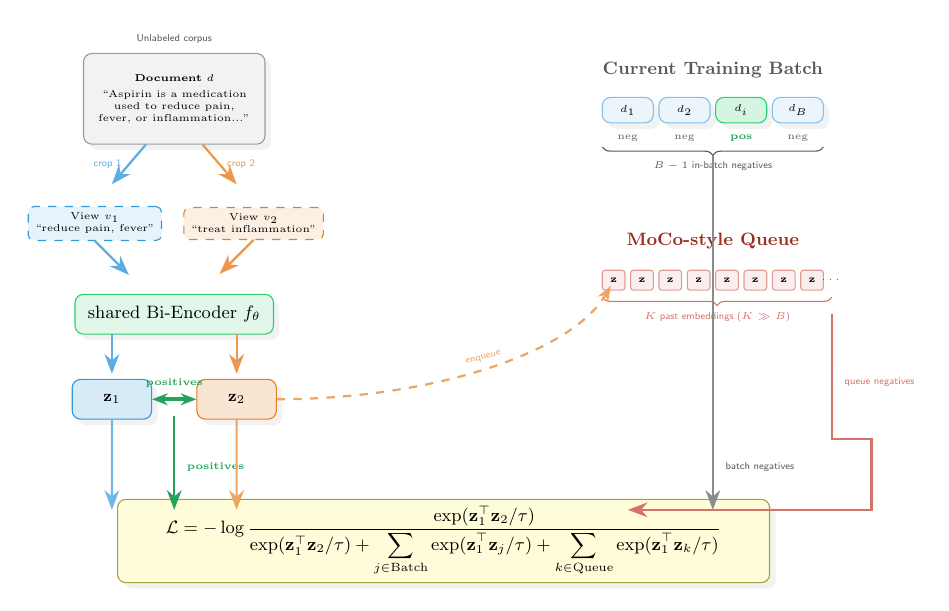
\begin{tikzpicture}[
    scale=0.72, transform shape,
    box/.style={draw, rounded corners=3pt, minimum height=0.7cm, align=center, font=\small, drop shadow={opacity=0.1}},
    arr/.style={-{Stealth[length=2.5mm]}, thick},
    crop/.style={draw, dashed, rounded corners=2pt, minimum height=0.55cm, font=\tiny, align=center},
]

% ===== LEFT COLUMN (x=0 area): Contrastive Pair Generation =====

% Original document
\node[box, fill=irInfra!8, draw=irInfra!60, minimum width=3.2cm, minimum height=1.6cm, font=\tiny, text width=2.8cm] (doc) at (0, 0)
    {\textbf{Document $d$}\\[2pt]
     ``Aspirin is a medication used to reduce pain, fever, or inflammation...''};
\node[font=\tiny\sffamily, text=irInfra, above=0.05cm of doc] {Unlabeled corpus};

% Two crop arrows
\draw[arr, draw=irSparse!80] ([xshift=-0.5cm]doc.south) -- ++(-0.6, -0.7)
    node[midway, left, font=\tiny\sffamily, text=irSparse!80] {crop 1};
\draw[arr, draw=irDense!80] ([xshift=0.5cm]doc.south) -- ++(0.6, -0.7)
    node[midway, right, font=\tiny\sffamily, text=irDense!80] {crop 2};

% View 1
\node[crop, fill=irSparse!12, draw=irSparse, minimum width=2.2cm] (v1) at (-1.4, -2.2)
    {View $v_1$\\``reduce pain, fever''};

% View 2
\node[crop, fill=irDense!12, draw=irDense, minimum width=2.2cm] (v2) at (1.4, -2.2)
    {View $v_2$\\``treat inflammation''};

% Encoder
\draw[arr, draw=irSparse!80] (v1.south) -- ++(0.6, -0.6);
\draw[arr, draw=irDense!80] (v2.south) -- ++(-0.6, -0.6);

\node[box, fill=irHybrid!15, draw=irHybrid, minimum width=3.5cm] (enc) at (0, -3.8)
    {shared Bi-Encoder $f_\theta$};

% Embeddings
\draw[arr, draw=irSparse!80] (-1.1, -4.15) -- (-1.1, -4.85);
\draw[arr, draw=irDense!80] (1.1, -4.15) -- (1.1, -4.85);

\node[box, fill=irSparse!20, draw=irSparse, minimum width=1.4cm, font=\footnotesize] (e1) at (-1.1, -5.3)
    {$\mathbf{z}_1$};
\node[box, fill=irDense!20, draw=irDense, minimum width=1.4cm, font=\footnotesize] (e2) at (1.1, -5.3)
    {$\mathbf{z}_2$};

% Pull together
\draw[irHybrid!80!black, ultra thick, {Stealth[length=2mm]}-{Stealth[length=2mm]}]
    (e1.east) -- (e2.west)
    node[midway, above=2pt, font=\tiny\bfseries, text=irHybrid!80!black] {positives};

% ===== RIGHT COLUMN (x=9.5 area): Negative Sources =====

% Current batch
\node[font=\small\bfseries, text=irInfra] at (9.5, 0.5) {Current Training Batch};
\foreach \i/\label/\type in {1/$d_1$/neg, 2/$d_2$/neg, 3/$d_i$/pos, 4/$d_B$/neg}{
    \pgfmathsetmacro{\xpos}{8.0 + (\i-1)*1.0}
    \ifnum\i=3
        \node[box, fill=irHybrid!20, draw=irHybrid, minimum width=0.9cm, minimum height=0.45cm, font=\tiny] (b\i) at (\xpos, -0.2) {\label};
        \node[font=\tiny\bfseries, text=irHybrid!80!black] at (\xpos, -0.7) {\type};
    \else
        \node[box, fill=irSparse!10, draw=irSparse!60, minimum width=0.9cm, minimum height=0.45cm, font=\tiny] (b\i) at (\xpos, -0.2) {\label};
        \node[font=\tiny, text=irInfra] at (\xpos, -0.7) {\type};
    \fi
}

% Brace for batch
\draw[decorate, decoration={brace, amplitude=3pt, mirror}, irInfra]
    (7.55, -0.85) -- (11.45, -0.85)
    node[midway, below=4pt, font=\tiny\sffamily, text=irInfra] {$B-1$ in-batch negatives};

% MoCo Queue
\node[font=\small\bfseries, text=irRerank!80!black] at (9.5, -2.5) {MoCo-style Queue};

% Queue slots
\foreach \i in {0,...,7}{
    \pgfmathsetmacro{\xpos}{7.75 + \i*0.5}
    \node[draw=irRerank!50, fill=irRerank!8, rounded corners=1pt, minimum width=0.4cm, minimum height=0.35cm, font=\tiny] (q\i) at (\xpos, -3.2) {$\mathbf{z}$};
}
\node[font=\tiny, text=irInfra] at (11.6, -3.2) {$\cdots$};

\draw[decorate, decoration={brace, amplitude=3pt, mirror}, irRerank!70]
    (7.55, -3.5) -- (11.6, -3.5)
    node[midway, below=4pt, font=\tiny\sffamily, text=irRerank!70] {$K$ past embeddings ($K \gg B$)};

% Enqueue arrow - redesigned to avoid crossings
\draw[arr, draw=irDense!70, dashed, -{Stealth[length=2mm]}] (e2.east) .. controls (4.5, -5.3) and (7.0, -4.5) .. (7.7, -3.3)
    node[pos=0.5, above, font=\tiny\sffamily, text=irDense!70, rotate=15] {enqueue};

% ===== BOTTOM AREA (x=4.5 area): Contrastive Loss =====

\node[box, fill=yellow!15, draw=yellow!60!black, minimum width=11.5cm, minimum height=1.1cm, font=\small] (loss) at (4.75, -7.8)
    {$\mathcal{L} = -\log \dfrac{\exp(\mathbf{z}_1^\top \mathbf{z}_2 / \tau)}{\exp(\mathbf{z}_1^\top \mathbf{z}_2 / \tau) + \displaystyle\sum_{j \in \text{Batch}} \exp(\mathbf{z}_1^\top \mathbf{z}_j / \tau) + \sum_{k \in \text{Queue}} \exp(\mathbf{z}_1^\top \mathbf{z}_k / \tau)}$};

% Component arrows into loss - spread out and using named anchors
\pgfmathsetmacro{\lossTop}{-7.25}

% Positive contribution
\draw[arr, draw=irHybrid!80!black] (0, -5.6) -- (0, \lossTop);
\node[font=\tiny\bfseries, text=irHybrid!80!black, anchor=west] at (0.1, -6.5) {positives};

% Batch contribution
\draw[arr, draw=irInfra!70] (9.5, -1.0) -- (9.5, \lossTop);
\node[font=\tiny\sffamily, text=irInfra, anchor=west] at (9.6, -6.5) {batch negatives};

% Queue contribution
\draw[arr, draw=irRerank!70] (11.6, -3.8) |- (12.3, -6.0) |- (8.0, \lossTop);
\node[font=\tiny\sffamily, text=irRerank!70, anchor=west] at (11.7, -5.0) {queue negatives};

% Shared embeddings arrows
\draw[arr, draw=irSparse!70] (e1.south) -- (-1.1, \lossTop);
\draw[arr, draw=irDense!70] (e2.south) -- (1.1, \lossTop);

\end{tikzpicture}

\end{center}
\end{frame}

\begin{frame}{Why Contriever Works (and What It Does Not Fix)}
\begin{columns}[T]
\begin{column}{0.52\textwidth}
\textbf{Why it works}
\begin{itemize}
    \item Learns \textbf{domain-agnostic semantic similarity}.
    \item Trained on \textbf{diverse web text}, not one supervised benchmark.
    % \item Symmetric query/document encoder improves \textbf{zero-shot robustness}.
    % \item Stronger \textbf{recall} than earlier dense retrievers.
\end{itemize}
\end{column}

\begin{column}{0.44\textwidth}
\textbf{Limits}
\begin{itemize}
    \item Still not always best at \textbf{top-rank precision} (\textit{nDCG@10}).
    % \item Weak on \textbf{time-specific} domains (e.g., TREC-COVID).
    \item Long, argument-heavy documents remain hard (e.g., T{\'o}uch{\'e}).
\end{itemize}
\end{column}
\end{columns}

\vspace{0.8em}
\cpause

\begin{exampleblock}{Teaching takeaway}
Contriever shows that dense retrieval can generalize \textbf{without labels}:
\[
\text{better pretraining} > \text{more MS MARCO supervision}
\]
for zero-shot transfer.
\end{exampleblock}
\end{frame}

\begin{frame}[shrink=10]{Hybrid Retrieval: Dense + Sparse}
\begin{block}{Key Finding}
Combining BM25 and dense retrieval \textbf{outperforms either alone}.
\end{block}

\vspace{0.5em}

$$\text{score}_{\text{hybrid}}(q, d) = \alpha \cdot \text{score}_{\text{BM25}}(q,d) + (1-\alpha) \cdot \text{score}_{\text{dense}}(q,d)$$

\vspace{0.5em}

\begin{center}
\begin{tabular}{lc}
\toprule
\textbf{Method} & \textbf{NQ Top-20 Recall} \\
\midrule
BM25 alone & 62.9 \\
DPR alone & 78.4 \\
BM25 + DPR (hybrid) & \textbf{82.6} \\
\bottomrule
\end{tabular}
\end{center}

\cpause
\vspace{0.5em}

\begin{exampleblock}{Why Hybrid Works}
Sparse captures \textbf{exact matches} (named entities, rare terms). Dense captures \textbf{semantic similarity} (paraphrases). They are complementary, not competing.
\end{exampleblock}
\end{frame}

\begin{frame}{Score-Agnostic Fusion: Reciprocal Rank Fusion}
\begin{block}{The Challenge}
Dense scores (dot products) and Sparse scores (BM25) are on \textbf{different scales}. How to combine them without fragile hyperparameter tuning?
\end{block}

\vspace{0.5em}

\begin{center}
% RRF: Reciprocal Rank Fusion Visualization
% Shows two ranked lists and their merged result based on ranks
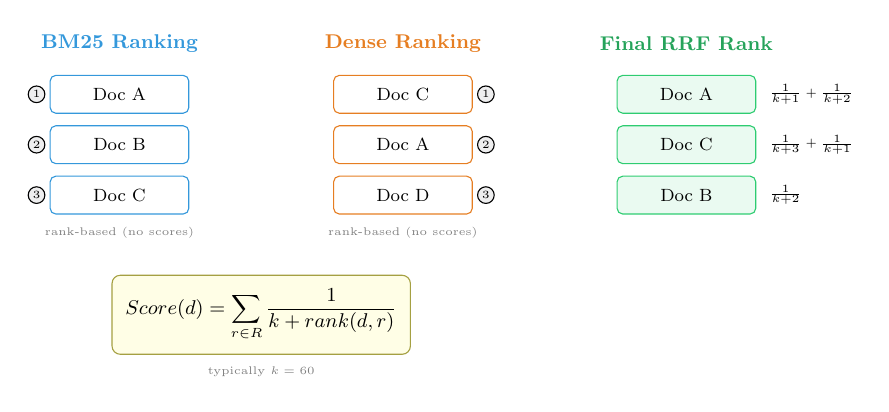
\begin{tikzpicture}[
    scale=0.8, transform shape,
    doc/.style={draw, rounded corners=2pt, minimum width=2.2cm, minimum height=0.6cm, font=\footnotesize, align=center, fill=white},
    rank/.style={circle, draw, inner sep=1pt, font=\tiny, fill=irInfra!10},
    formula/.style={draw=yellow!60!black, fill=yellow!10, rounded corners=3pt, inner sep=6pt, font=\small}
]

% ===== LIST 1 (BM25) =====
\node[font=\small\bfseries, text=irSparse] at (0, 0.8) {BM25 Ranking};
\node[doc, draw=irSparse] (L1_1) at (0, 0) {Doc A}; \node[rank, left=2pt of L1_1] {1};
\node[doc, draw=irSparse] (L1_2) at (0, -0.8) {Doc B}; \node[rank, left=2pt of L1_2] {2};
\node[doc, draw=irSparse] (L1_3) at (0, -1.6) {Doc C}; \node[rank, left=2pt of L1_3] {3};
\node[font=\tiny, gray] at (0, -2.2) {rank-based (no scores)};

% ===== LIST 2 (Dense) =====
\node[font=\small\bfseries, text=irDense] at (4.5, 0.8) {Dense Ranking};
\node[doc, draw=irDense] (L2_1) at (4.5, 0) {Doc C}; \node[rank, right=2pt of L2_1] {1};
\node[doc, draw=irDense] (L2_2) at (4.5, -0.8) {Doc A}; \node[rank, right=2pt of L2_2] {2};
\node[doc, draw=irDense] (L2_3) at (4.5, -1.6) {Doc D}; \node[rank, right=2pt of L2_3] {3};
\node[font=\tiny, gray] at (4.5, -2.2) {rank-based (no scores)};

% ===== MERGING PROCESS =====
\node[formula] (eq) at (2.25, -3.5) {$Score(d) = \displaystyle\sum_{r \in R} \frac{1}{k + rank(d, r)}$};
\node[font=\tiny, below=2pt of eq, gray] {typically $k=60$};

% ===== FINAL RANKING =====
\node[font=\small\bfseries, text=irHybrid!80!black] at (9, 0.8) {Final RRF Rank};

% Doc A: 1/61 + 1/62
\node[doc, fill=irHybrid!10, draw=irHybrid] (M1) at (9, 0) {Doc A}; 
\node[font=\tiny, anchor=west] at (M1.east) {\ $\frac{1}{k+1} + \frac{1}{k+2}$};

% Doc C: 1/63 + 1/61
\node[doc, fill=irHybrid!10, draw=irHybrid] (M2) at (9, -0.8) {Doc C};
\node[font=\tiny, anchor=west] at (M2.east) {\ $\frac{1}{k+3} + \frac{1}{k+1}$};

% Doc B: 1/62
\node[doc, fill=irHybrid!10, draw=irHybrid] (M3) at (9, -1.6) {Doc B};
\node[font=\tiny, anchor=west] at (M3.east) {\ $\frac{1}{k+2}$};

\end{tikzpicture}

\end{center}

\vspace{0.5em}
\cpause

\begin{alertblock}{Reciprocal Rank Fusion (RRF)}
RRF relies only on \textbf{rankings}. It favors documents that appear high in \textit{any} characteristic (sparse or dense).
\end{alertblock}
\end{frame}

% ====================================================================
\section{Retrieval-Augmented Generation (RAG)}
% ====================================================================

\begin{frame}[plain]
\sectionpage
\end{frame}

\begin{frame}{Beyond Ranking: Retrieval-Augmented Generation (RAG)}
\begin{block}{The Paradigm Shift}
In modern AI applications, retrieval is not the final step. It is the \textbf{foundation} for Large Language Models (LLMs).
\end{block}

\vspace{1em}
\cpause

\begin{itemize}
    \item \textbf{Problem:} LLMs hallucinate and have a fixed knowledge cutoff.
    \item \textbf{Solution:} Retrieve relevant, up-to-date passages and provide them as \textbf{grounding context} in the model's prompt.
    \item \textbf{Impact:} Retrieval expands the model's memory and enables it to cite its sources.
\end{itemize}
\end{frame}

\begin{frame}[fragile]{The Modern IR Pipeline with RAG}
\begin{center}
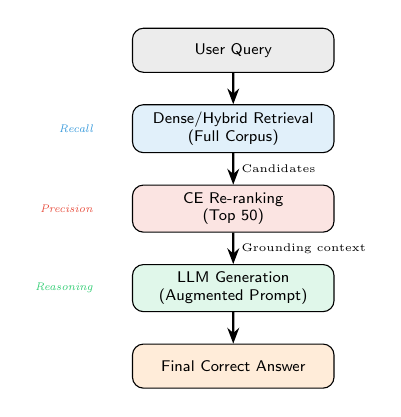
\begin{tikzpicture}[
    scale=0.8, transform shape,
    box/.style={draw, rounded corners, fill=#1, minimum height=0.7cm, minimum width=3.2cm, align=center, font=\scriptsize\sffamily},
    arr/.style={-{Stealth[length=2mm]}, thick}
]
\node[box=gray!15] (q) {User Query};
\node[box=sparse!15, below=0.5cm of q] (ret) {Dense/Hybrid Retrieval\\(Full Corpus)};
\node[box=dense!15, below=0.5cm of ret] (rr) {CE Re-ranking\\(Top 50)};
\node[box=hybrid!15, below=0.5cm of rr] (rag) {LLM Generation\\(Augmented Prompt)};
\node[box=orange!15, below=0.5cm of rag] (ans) {Final Correct Answer};

\draw[arr] (q) -- (ret);
\draw[arr] (ret) -- (rr) node[midway, right, font=\tiny] {Candidates};
\draw[arr] (rr) -- (rag) node[midway, right, font=\tiny] {Grounding context};
\draw[arr] (rag) -- (ans);

\node[left=0.5cm of ret, font=\tiny\itshape, text=sparse] {Recall};
\node[left=0.5cm of rr, font=\tiny\itshape, text=dense] {Precision};
\node[left=0.5cm of rag, font=\tiny\itshape, text=hybrid] {Reasoning};
\end{tikzpicture}
\end{center}

\vspace{0.5em}
\cpause

\begin{block}{Retrieval as the "Eyes" of the LLM}
If the retriever (bi-encoder) or re-ranker (cross-encoder) fails, the generator \textbf{cannot} produce a factual answer. High-quality IR is the bottleneck for RAG accuracy.
\end{block}
\end{frame}


% ====================================================================
\section{Connections and Summary}
% ====================================================================

\begin{frame}[plain]
\sectionpage
\end{frame}

\begin{frame}[fragile]{The Complete Modern Retrieval Stack}
\begin{center}
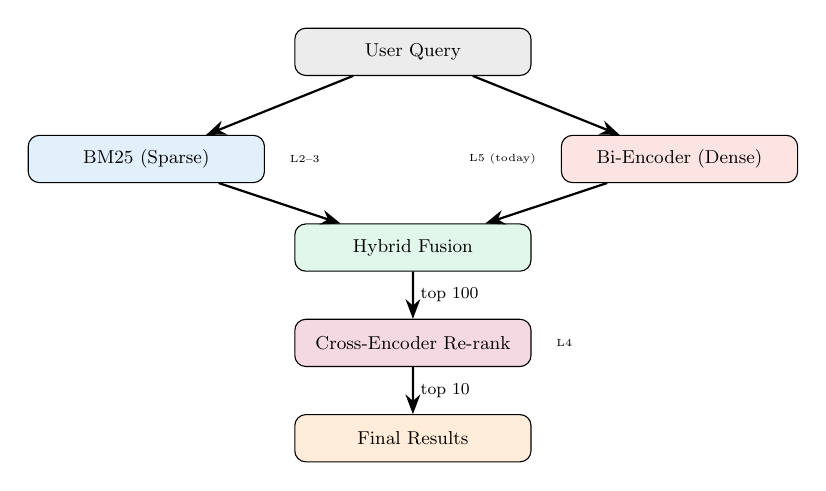
\begin{tikzpicture}[
    scale=0.75, transform shape,
    box/.style={draw, rounded corners, fill=#1, minimum height=0.8cm, minimum width=4cm, align=center, font=\small},
    arr/.style={-{Stealth[length=2.5mm]}, thick}
]
\node[box=gray!15] (query) {User Query};
\node[box=sparse!15, below left=1cm and 0.5cm of query] (bm25) {BM25 (Sparse)};
\node[box=dense!15, below right=1cm and 0.5cm of query] (dense) {Bi-Encoder (Dense)};
\node[box=hybrid!15, below=2.5cm of query] (fuse) {Hybrid Fusion};
\node[box=purple!15, below=0.8cm of fuse] (ce) {Cross-Encoder Re-rank};
\node[box=orange!15, below=0.8cm of ce] (result) {Final Results};

\draw[arr] (query) -- (bm25);
\draw[arr] (query) -- (dense);
\draw[arr] (bm25) -- (fuse);
\draw[arr] (dense) -- (fuse);
\draw[arr] (fuse) -- (ce) node[midway, right, font=\footnotesize] {top 100};
\draw[arr] (ce) -- (result) node[midway, right, font=\footnotesize] {top 10};

\node[font=\tiny, right=0.3cm of bm25] {L2--3};
\node[font=\tiny, left=0.3cm of dense] {L5 (today)};
\node[font=\tiny, right=0.3cm of ce] {L4};
\end{tikzpicture}
\end{center}

\vspace{0.3em}

Each lecture adds a component. Dense retrieval (today) gives us semantic first-stage retrieval --- the missing piece from Lecture 4.
\end{frame}

\begin{frame}[plain]
\sectionpage
\end{frame}

\begin{frame}[shrink=5]{Key Takeaways}
\begin{block}{1. Bi-Encoders Enable Semantic Retrieval at Scale}
Encode documents offline, search with ANN indexes from Lecture 2. Solves the vocabulary mismatch problem that BM25 cannot.
\end{block}

\begin{block}{2. Contrastive Learning Is the Training Paradigm}
InfoNCE loss with in-batch negatives. Larger batches = more negatives = better training. Temperature $\tau$ is a critical hyperparameter.
\end{block}

\begin{block}{3. DPR $\to$ ColBERT $\to$ ANCE: Improving Dense Retrieval}
DPR: single-vector bi-encoder. ColBERT: token-level late interaction. ANCE: dynamic hard negatives via asynchronous index refresh.
\end{block}

\begin{block}{4. Hybrid Retrieval Is the Practical Standard}
Dense + sparse complementary. BM25 for exact match, dense for semantics. Cross-encoder on top for final precision.
\end{block}
\end{frame}


\begin{frame}{Questions?}
\begin{center}
\Huge Questions?

\normalsize
\vspace{1em}
\textbf{Preview:} Next class we solve the \textit{Recall Ceiling} with \textbf{Dense Retrieval}.
\end{center}
\end{frame}























% ====================================================================
% APPENDIX / BACKUP SLIDES
% ====================================================================
\appendix






\end{document}
